\documentclass{article}

\usepackage[left=2cm,right=2cm, top=2cm, bottom = 2cm]{geometry}
\usepackage{amsfonts}

\usepackage{amsmath}
\usepackage{xcolor}

\usepackage{tikz}
\usepackage{subfigure}



\pagestyle{empty}

\setlength{\tabcolsep}{15pt}


\newcommand{\deriv}[3][]{\frac{\mathrm{d}^{#1}#2}{\mathrm{d}#3^{#1}}}
\newcommand{\diff}{\;\mathrm{d}}

\newcommand{\norm}[1]{\left|\kern-1pt\left|#1\right|\kern-1pt\right|}

\newcommand{\bra}[1]{\left\langle #1 \,\right|}
\newcommand{\ket}[1]{\left|\, #1\right\rangle}
\newcommand{\braket}[2]{\left\langle #1 \mid #2 \right\rangle}

\let\rarrow\overrightarrow


\begin{document}

\title{Inner Products and Vector Geometry}
\date{}

\maketitle
\thispagestyle{empty}

\vskip -10mm

\Large

\textbf{\underline{Objective: To understand how inner products relate to classical}}

\textbf{\underline{geometry.}}





\vspace{3mm}







\textbf{Warm-up: The Dot Product:}\bigskip


We work in two-dimensional real space, $\mathbb{R}^2$, with the usual dot product (Euclidean inner product):
\[u\cdot v = \norm{u}\times \norm{v}\times \cos(\theta),\]
where $\theta$ is the angle between $u$ and $v$.

We will prove that this definition of the dot product is equivalent to the other one we have seen, that $(u_1,u_2)\cdot(v_1,v_2)=u_1v_1+u_2v_2$. To do this, consider the diagram below.
\begin{enumerate}
	\item Write $u_1$ and $u_2$ in terms of $\alpha$ and $\norm{u}$.
	\item Write $v_1$ and $v_2$ in terms of $\beta$ and $\norm{v}$.
	\item Hence write $u_1v_1+u_2v_2$ in terms of $\norm{u}$, $\norm{v}$, $\alpha$, and $\beta$.
	\item Use a trigonometric identity and $\theta=\alpha-\beta$ to simplify your above expression and show that
		\[u_1v_1+u_2v_2=\norm{u}\times \norm{v}\times \cos(\theta).\]
\end{enumerate}

\begin{center}
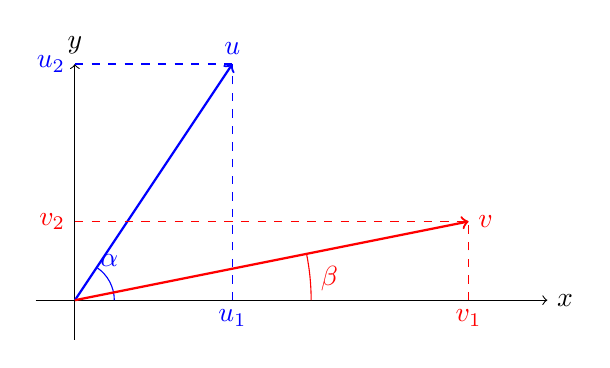
\begin{tikzpicture}
	\draw[->] (-0.5,0) -- (6,0);
	\node[right] at (6,0) {$x$};
	\draw[->] (0,-0.5) -- (0,3);
	\node[above] at (0,3) {$y$};
	
	\draw[blue,thick,->] (0,0) -- (2,3);
	\node[blue,above] at (2,3) {$u$};
	\draw[dashed,blue] (0,3) -- (2,3);
	\node[left,blue] at (0,3) {$u_2$};
	\draw[dashed,blue] (2,0) -- (2,3);
	\node[below,blue] at (2,0) {$u_1$};
	\draw[blue] (0.5,0) arc (0:56.31:0.5);
	\node[blue,right] at (0.2,0.5) {$\alpha$};
	
	\draw[red,thick,->] (0,0) -- (5,1);
	\node[red,right] at (5,1) {$v$};
	\draw[red,dashed] (0,1) -- (5,1);
	\node[left,red] at (0,1) {$v_2$};
	\draw[dashed,red] (5,0) -- (5,1);
	\node[below,red] at (5,0) {$v_1$};
	\draw[red] (3,0) arc (0:11.31:3);
	\node[red,above right] at (3,0) {$\beta$};
\end{tikzpicture}
\end{center}



\clearpage










\textbf{Theory: Inner Products and Geometry:}

\bigskip



Consider a right-angled triangle $ABC$:
\begin{center}
\begin{tikzpicture}[scale=0.5]
	\draw (0,0) -- (12,0) -- (12,5) -- (0,0);
	\node[below left] at (0,0) {$C$};
	\node[below right] at (12,0) {$A$};
	\node[right] at (12,5) {$B$};
\end{tikzpicture}
\end{center}

Let $u$ be the vector $\rarrow{BA}$ and $v$ be the vector $\rarrow{AC}$. Then $\rarrow{BC} = \rarrow{BA}+\rarrow{AC}=u+v$. So, by Pythagoras' Theorem,
\[\norm{u}^2+\norm{v}^2=\norm{u+v}^2.\]
The fact that $ABC$ is right-angled can be expressed by the fact that $\cos(\theta)=0$, where $\theta$ is the angle between $u$ and $v$. In other words, it is the fact that $u\cdot v=0$. So Pythagoras' Theorem can be expressed as a statement about the norms of orthogonal vectors in $\mathbb{R}^2$. We will now show that there is nothing special about $\mathbb{R}^2$ or the dot product here; a version of Pythagoras' Theorem holds for any inner product on any vector space!

So suppose that $u$ and $v$ are vectors in some vector space, and we have an inner product, such that $u$ and $v$ are orthogonal: $\braket{u}{v}=0$. Then
\begin{align*}
	\norm{u+v}^2 &= \braket{u+v}{u+v}\\
	&=\braket{u}{u+v} + \braket{v}{u+v}\\
	&= \braket{u}{u} + \braket{u}{v} + \braket{v}{u} + \braket{v}{v}\\
	&= \braket{u}{u} + 2 \braket{u}{v} + \braket{v}{v}\\
	&= \norm{u}^2 + 2(0) + \norm{v}^2\\
	&= \norm{u}^2+\norm{v}^2.
\end{align*}\medskip


Example: Take $L_2([0,2\pi])$, the vector space of square-integrable functions from $[0,2\pi]$ to $\mathbb{R}$, with inner product given by
\[\braket{f}{g}=\frac{1}{\pi}\int_0^{2\pi}f(x)g(x)\diff x.\]
Then $\cos(x)$ and $\sin(x)$ are orthonormal (exercise), so $\braket{\cos(x)}{\sin(x)}=0$ and $\norm{\cos(x)}=\norm{\sin(x)}=1$; so we should have
\[\norm{\cos(x)+\sin(x)}=\sqrt{1^2 +1^2}=\sqrt{2}.\]
Check that this is indeed true.




\clearpage












\textbf{Theory: The Cauchy-Schwarz Inequality:}

\bigskip

One of the most important results in the theory of inner products is the \textbf{Cauchy-Schwarz inequality}:
\[\left|\braket{u}{v}\right|\leq \norm{u}\norm{v}.\]

To prove this, we let $\lambda=\frac{\braket{u}{v}}{\norm{v}^2}$ and note that
\begin{align*}
	0\leq \norm{u-\lambda v}^2&= \braket{u-\lambda v}{u-\lambda v}\\
	&= \braket{u}{u} -2\lambda\braket{u}{v} + \lambda^2 \braket{v}{v}\\
	&= \norm{u}^2 -2\lambda\braket{u}{v}+\lambda^2\norm{v}^2\\
	&=\norm{u}^2 - 2\frac{\braket{u}{v}^2}{\norm{v}^2} + \frac{\braket{u}{v}^2}{\norm{v}^2}\\
	&= \norm{u}^2 -\frac{\braket{u}{v}^2}{\norm{v}^2}.
\end{align*}
Rearranging and multiplying through by $\norm{v}^2$, we get
\[\braket{u}{v}\leq \norm{u}^2\norm{v}^2.\]
Taking square roots then completes the proof.\bigskip

A key consequence of the Cauchy-Schwarz inequality is that
\[-1\leq \frac{\braket{u}{v}}{\norm{u}\norm{v}}\leq 1.\]
This means that we can take the arccosine of this expression; so we define the \textbf{angle between two vectors} $u$ and $v$ to be
\[\theta=\cos^{-1}\left(\frac{\braket{u}{v}}{\norm{u}\norm{v}}\right).\]
This means that it is true \textit{by definition} that $\braket{u}{v}=\norm{u}\norm{v}\cos(\theta)$, where $\theta$ is the angle between $u$ and $v$.\bigskip

Note that the angle $\theta$ might not have any clear geometric meaning. Some vector spaces with inner products, such as $L_2([0,2\pi])$, are massively infinite-dimensional, so we cannot possibly visualise them, or what the angle between two functions means. However, we can reason by analogy with geometry in $\mathbb{R}^2$ and $\mathbb{R}^3$ to make ``geometric'' statements about any vector space with an inner product on it. Essentially, the significance of Cauchy-Schwarz is that it lets us do classical geometry in any inner product space.

In particular, given a vector $v$, we can talk about its length $\norm{v}$ and the angle it makes with any other vector $u$. So we can describe the magnitude and direction of $v$. The standard intuitive description of a vector at school or in physics courses is that a vector is something with magnitude and direction; in fact, this is not true. Rather, \textit{once you have an inner product}, a vector is something with a magnitude and direction, but if you have a vector space with no inner product on it, you cannot meaningfully talk about magnitude or direction of vectors. It's just that the vector spaces of most interest in physics are $\mathbb{R}^n$, which have a standard inner product on them (the dot product), and $\mathbb{C}^n$, which has a standard inner product too (essentially also the dot product, but with a complex conjugation thrown in to make it positive-definite).\bigskip


Classic results of geometry like the cosine rule follow straightforwardly from the definition of the angle between two vectors by Cauchy-Schwarz. In $\mathbb{R}^2$, the cosine rule says that if we have vectors $u$ and $v$, so that $u$, $v$, and $u-v$ are the edges of a triangle, then
\[\norm{u-v}^2=\norm{u}^2+\norm{v}^2-2\norm{u}\norm{v}\cos(\theta),\]
where $\theta$ is the angle between $u$ and $v$. In terms of the inner product, this equation becomes
\[\braket{u-v}{u-v}=\braket{u}{u}+\braket{v}{v}-2\braket{u}{v},\]
which is easily found to be true for any vectors $u$ and $v$ from the linearity properties of the inner product. So the cosine rule still holds in any inner product space.\bigskip


It is worth saying something about the proof of Cauchy-Schwarz given above. It probably seems very mysterious; where does the definition of $\lambda$ come from? Why consider $\norm{u-\lambda v}^2$? If we think about the expression $u-\lambda v$ in $\mathbb{R}^2$, where $\lambda=\frac{u\cdot v}{\norm{v}^2}$, we see that 
\begin{align*}
	u-\lambda v &= u-\frac{\norm{u}\norm{v}\cos(\theta)}{\norm{v}^2}v\\
	&=u-\norm{u}\cos(\theta)\hat{v},
\end{align*}
where $\hat{v}=\frac{v}{\norm{v}}$ is the unit vector in the direction of $v$. By SohCahToa, $\norm{u}\cos(\theta)$ is the projection of $u$ in the direction of $v$; so we are subtracting from $u$ precisely the component of $u$ in the direction of $v$. The diagram should clarify this:

\begin{center}
\begin{tikzpicture}
	\draw[->,thick] (0,0) -- (3,0);
	\node[right] at (3,0) {$v$};
	\draw[->,thick] (0,0) -- (2,4);
	\node[above] at (2,4) {$u$};
	
	\draw[thick,red,->] (0,0) -- (1,0);
	\node[red,below] at (1,0) {$\hat{v}$};
\end{tikzpicture}
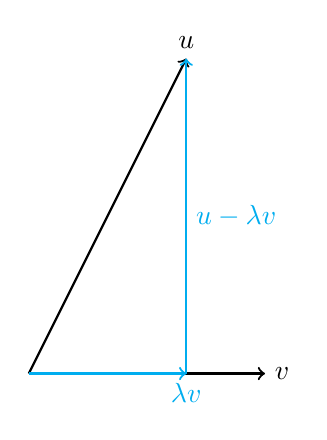
\begin{tikzpicture}
	\draw[->,thick] (0,0) -- (3,0);
	\node[right] at (3,0) {$v$};
	\draw[->,thick] (0,0) -- (2,4);
	\node[above] at (2,4) {$u$};
	
	\draw[cyan,thick,->] (0,0) -- (2,0);
	\node[cyan,below] at (2,0) {$\lambda v$};
	\draw[cyan,thick,->] (2,0) -- (2,4);
	\node[right,cyan] at (2,2) {$u-\lambda v$};
\end{tikzpicture}
\end{center}

So $u=(u-\lambda v)+\lambda v$ and $u-\lambda v$ is orthogonal (perpendicular) to $v$. So we are resolving $u$ into components parallel to $v$ and perpendicular to $v$, and so $\norm{u-\lambda v}$ is the length of the component of $u$ perpendicular to $v$. This makes sense in $\mathbb{R}^2$ (or $\mathbb{R}^n$), and then our proof of Cauchy-Schwarz uses this idea and considers $\norm{u-\lambda v}$.

From the diagram, by Pythagoras' Theorem, we expect
\[\norm{u-\lambda v}^2=\norm{u}^2-\norm{\lambda v}^2.\]
Indeed, this is exactly what we find from the algebraic manipulations. So even though, \textit{a priori}, the geometric diagram has no meaning in an abstract inner product space, algebraically the proof inspired by the geometry still works.

Then, once the proof is complete and we use Cauchy-Schwarz to define the angle between two vectors in a general inner product space, we can go back and see that we can now \textit{literally} regard $u-\lambda v$ as being the component of $u$ perpendicular to $v$---so we use an idea from geometry to prove Cauchy-Schwarz, then use Cauchy-Schwarz to allow us to do geometry in any inner product space, so our geometry-inspired proof of Cauchy-Schwarz actually (in a somewhat circular way) becomes a literally geometric proof! Crucially, however, although geometry \textit{inspired} the proof of Cauchy-Schwarz, the proof itself works without any reference to geometry (it just would be rather harder to think of!). So there is no logical circularity, and the proof is valid.




\end{document}